\documentclass[12pt]{article}

%useful packages
\usepackage{color,soul}
\usepackage[usenames,dvipsnames,svgnames,table]{xcolor}
\usepackage{amsmath,amsthm,amscd,amssymb,bm}
\usepackage{hyperref}
\hypersetup{
    colorlinks=true,
    linkcolor=JungleGreen,
    urlcolor  =JungleGreen,
    citecolor = JungleGreen,
    anchorcolor = JungleGreen
}
\usepackage[utf8]{inputenc}
\usepackage[top=2cm, bottom=3cm, left=2cm, right=2cm]{geometry}
\usepackage{pgfplots}
\usepackage{enumitem}
\usepgfplotslibrary{fillbetween}
\usetikzlibrary{patterns}
\usepackage{tcolorbox}
\usepackage{centernot}
\usepackage{mathtools}
\usepackage{xcolor}

%personal definitions and commands
\newcommand{\R}{\mathbb{R}} 
\newcommand{\E}{\mathbb{E}}
\newcommand{\V}{\mathbb{V}}
\newcommand{\C}{\mathbb{C}}
\newcommand{\Prob}{\mathbb{P}}
\newcommand{\e}{\epsilon}
\newcommand\numberthis{\addtocounter{equation}{1}\tag{\theequation}} %allows numbering of single equations in align* environment
\newcommand{\mtx}[1]{\ensuremath{\bm{\mathit{#1}}}}
\newcommand{\B}{\hat{\boldsymbol{\beta}}}
\newcommand{\Cov}{\mathbb{C}\text{ov}}
\newcommand{\N}{\mathcal{N}}



\title{Replication of `The Power of Forward Guidance Revisited' by McKay, Nakamura \& Steinnson (2016)}
\author{Anirudh Yadav}
\setlength\parindent{0pt}
\begin{document}

\maketitle

\setcounter{tocdepth}{2}
\tableofcontents

\newpage

\section{Overview}
In the basic New Keynesian model (NKM) studied in class the output and inflation response to forward guidance is implausibly large. A potential reason for this `forward guidance puzzle' is the complete markets assumption, which allows the representative agent to take full advantage of any opportunity to intertemporally substitute consumption. McKay, Nakamura and Steinnson's (2016, henceforth MNS) main question is whether the output response to forward guidance is smaller in a NKM with idiosyncratic income risk and incomplete markets. It turns out that it is. The main intuition for their result is that in the model with incomplete markets agents exhibit precautionary savings behaviour. The desire to save for bad times mitigates agents' desire to move consumption forward, dampening the aggregate output response relative to the basic NKM.

\section{Forward guidance in the basic New Keynesian Model}
The first part of the paper shows why forward guidance is so powerful in the basic NKM. Consider the plain vanilla NKM studied in class:
\begin{align*}
y_t &= \E_t[y_{t+1}] - \sigma(i_t - \E_t[\pi_{t+1}] - r_t^n) &\text{ `NK IS curve'}\\
\pi_t  &= \beta\E_t[\pi_{t+1}]  + \kappa y_t &\text{ `NKPC'}
\end{align*}
where the variables have the usual interpretation. Next, suppose the monetary policy rule is given by
\begin{align*}
r_t = i_t - \E_t[\pi_{t+1}] = r_t^n + \e_{t,t-j},
\end{align*}
where $\e_{t,t-j}$ is a monetary shock in period $t$ that is announced in period $t-j$. Suppose the economy starts in steady state and the central bank announces that the real rate will be lower by 1 percentage point for a single quarter, one year in the future; i.e. $\e_{t+4,t} = -0.01.$ To implement this type of shock in AIM, I add the following $MA$ state variables (as discussed in class) to the standard setup:
\begin{align*}
\tilde{r}_t \equiv r_t - r_t^n &= a_1MA_t^1 + a_2MA_t^2 + a_2MA_t^3 + a_4MA_t^4 + a_5MA_t^5
\end{align*}
with
\begin{align*}
MA_t^1 &= \e_{t+4,t}=
\begin{cases}
-0.01 &\text{ if } t=1 \\
0 &\text{ otherwise.}
\end{cases}
\end{align*} 
and
\begin{align*}
MA^j_t = MA_{t-1}^{j-1}
\end{align*}
and $a_1=a_2=a_3=a_4=0$, $a_5 = 1$.\\

Figure 1 plots the response of the output gap to this shock for $\sigma=1$ (other parameter values are standard), replicating Figure 1 in MNS. To understand why the output response is so big, consider the representative agent's linearized Euler equation:
\begin{align*}
\E_t[\Delta\tilde{c}_{t+1}] = \beta \tilde{r}_t 
\end{align*}
which dictates that consumption moves in lock-step with the real rate. Accordingly, with no borrowing constraint, the representative agent can take full advantage of the opportunity to intertemporally substitute.

\begin{figure}[htpb!]
 \centering
 	\caption{Response of Output to Forward Guidance in the Basic NKM}
        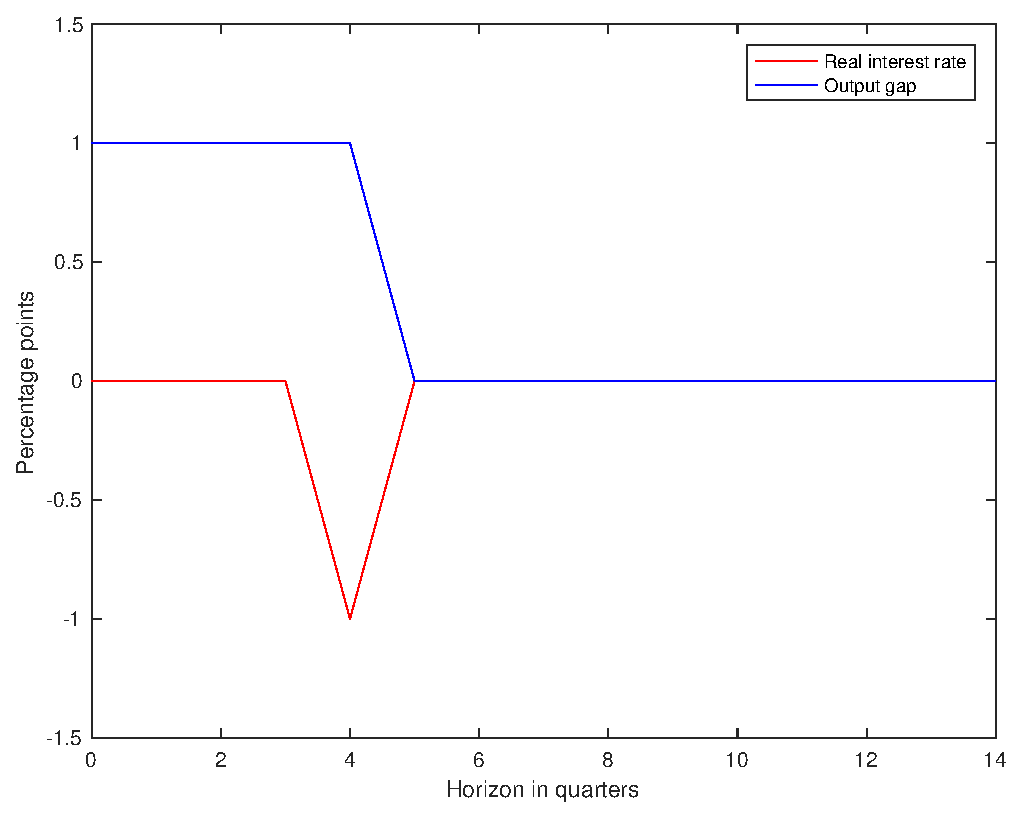
\includegraphics[width=0.7\textwidth]{IR_1_R.eps}
\end{figure}



\section{MNS's model}
MNS's model is essentially the basic NKM combined with the main elements of the Huggett model.

\subsection{Households}
There are a continuum of households indexed by $h$. The households' problem is
\begin{align*}
&\max_{\{c,\ell, b_{t+1}\}} \E_0\sum_{t=0}^\infty \beta^t \left(\frac{c_{h,t}^{1-\gamma}}{1-\gamma} - \frac{\ell_{h,t}^{1+\psi}}{1+\psi}\right)\\
\\
&\text{s.t. } c_{h,t} + \frac{b_{h,t+1}}{1+r_t} = b_{h,t} + W_tz_{h,t}\ell_{h,t} - \tau_t\bar\tau(z_{h,t}) +D_t\\
\\
&\text{\& } b_{h,t+1} \geq 0.
\end{align*}
where $z_{h,t}$ is the household's idiosyncratic productivity, which follows a Markov chain with transition probabilities $\Pr(z_{h,t+1}|z_{h,t})$. Households are taxed according to their labor productivity and each receives an equal dividend $D_t$ from intermediate goods firms. Other variables have the standard interpretation.

\subsection{Production}
The production side of the economy is almost identical to the basic NKM studied in class so I suppress the details for brevity. The only differences from the NKM studied in class are: (i) there is no capital; and (ii) intermediate goods firms have linear production technology in labor.

\subsection{Government}
The government runs a balanced budget to maintain a level of debt $B$ each period. The government's budget constraint is
\begin{align*}
\frac{B}{1+r_t} + \sum_z \Gamma^z(z)\tau_t\bar\tau(z) = B
\end{align*}
where $\Gamma^z$ is invariant cross-sectional distribution of productivities. The government is not very important for the model: it simply provides a saving vehicle for households, and taxes the required amount in order to pay interest on its debt.

\subsection{Equilibrium}
I outline the main equilibrium conditions of the model below. The aggregate production function is 
\begin{align*}
S_tY_t = \int n_{j,t}dj \equiv N_t
\end{align*} 
where $j$ indexes the intermediate goods producers, $N_t$ is aggregate labor demand, and $S_t \equiv \int_0^1 \left(\frac{p_{j,t}}{P_t}\right)^{\mu/(1-\mu)}$ where $\mu$ is the elasticity of substitution across intermediate goods as usual. $S_t$ evolves according to equation (10) in MNS.\\

Aggregate labor market clearing requires
\begin{align*}
L_t \equiv \int z\ell_t(z,b) d\Gamma_t(z,b) = N_t
\end{align*}
where $L_t$ is aggregate labor supply, $\ell_t(z,b)$ is the household's decision rule for labor, and $\Gamma(z,b)$ is the distribution of households over idiosyncratic states. \\

Bond market clearing requires
\begin{align*}
B = \int b_t(z,b)d\Gamma_t(z,b)
\end{align*}
where $g_t(z,b)$ is the household's decision rule for savings. \\

The aggregate dividend is given by
\begin{align*}
D_t = Y_t - W_tN_t.
\end{align*}
And finally, goods market clearing requires
\begin{align*}
C_t \equiv \int g_t(z,b)d\Gamma_t(z,b) = Y_t,
\end{align*}
where $g_t(z,b)$ is the household's decision rule for consumption.\\

Equilibrium has the standard definition, which I omit for brevity.

\subsection{Calibration}
MNS calibrate the idiosyncratic productivity to match the persistent component of estimated AR(1) wage process in Floden and Linde (2001). Their basline calibration results in a 3-point Markov chain with transition matrix:
\begin{align*}
\mtx{P} = 
\begin{bmatrix}
0.966 &	0.0338 &	0.00029 \\
0.017&	0.966& 	0.017 \\
0.0003 &	0.0337 &	0.966
\end{bmatrix}
\end{align*} 
and a vector of state values given by $Z = \{0.492,1,2.031\} \equiv \{z_l, z_m, z_h\}$. The supply of government bonds, $B$, is calibrated to 1.4 $\times$ annual GDP; since the time period for the model is one quarter, this calibration implies $B = 1.4 \times 4 \times Y_t$.\footnote{This calibration seems to imply that $B$ is potentially time varying. However, in their setup the government maintains a constant level of assets. Accordingly, I'm not sure if I'm interpreting their calibration correctly.}. MNS also assume that only the most productive households pay tax, so that $\bar \tau(z_h) = 1$ and $\bar \tau(z)=0$ otherwise. Other parameter values are standard, and are summarized in Table 1 in MNS.

\section{Steady state}
Unfortunately, I was unable to get the transitional dynamics associated with forward guidance in MNS's model due to the time constraint. Accordingly, I focus on my solution for the steady state of MNS's model, which is not presented in their paper.

\subsection{Solving the household's problem}
The first ingredient that I need in order to solve for steady state is the household's policy function for consumption, which also pins down their savings and labor supply decisions. To solve for the policy function, I follow MNS and use the so-called `endogenous grid method' (EGM). I leave the details to the Appendix, but the basic idea of EGM is to iterate on the household's Euler equation. I start with an initial guess of the policy function $g^0(z,b)$. Then (assuming the household is not at the borrowing constraint) I can use the Euler equation to get optimal consumption today:
\begin{align*}
c^{-\gamma} = \beta(1+\bar r) \sum_{z'}\Pr(z'|z)(g^0(z',b'))^{-\gamma}.
\end{align*}
Next, I can use the intertemporal budget constraint to back out the level of bond holdings that the household must have had today, in order to finance this policy. It is also easy to identify which agents hit the borrowing constraint, in which case I use their budget constraint to determine consumption, rather than the Euler equation (see Appendix for details). \\

In summary, at every iteration EGM spits out an endogenous grid of bond holdings today, and an associated level of consumption, for each level of productivity. In order to map this policy back onto the original grid of bond holdings, I need to use some interpolation technique. I use a linear interpolation for simplicity, but MNS use a cubic spline.

\subsection{Simulating the distribution of bond holdings}
To simulate the distribution of bond holdings I first get a vector of 1 million idiosyncratic productivity draws, using the Markov chain above. I then use the household's policy function to get the level of bond holdings associated with each value of productivity. That is,
\begin{enumerate}
\item At time $t=0$, I set $z_0$ to $z_m \in Z$.
\item For each subsequent period $t+1$, the new state $z_{t+1}$ is drawn using $\mtx{P}$.
\item I then pick an initial level of bond holdings $b_0 = 0$.
\item For each subsequent period $t+1$, the new level of bond holdings is given by $$b_{t+1} = (1+\bar r)[b_t+(\bar{W}z_t)^{1+1/\psi}g(z_t,b_t)^{-\gamma/\psi}+\bar{D}-g(z_t,b_t)]. $$
\end{enumerate}


\subsection{The iterative procedure}
Before outlining my iterative procedure, I write down some useful steady state conditions. First, linear production technology implies that  $\bar Y = \bar N$. Thus, the steady state dividend is $\bar D = \bar Y (1-\bar W) = \bar C (1-\bar W)$. Next, note that the government's budget constraint implies
\begin{align*}
\sum_z \Gamma^z(z)\bar \tau\bar\tau(z) &= B\left[\frac{\bar r}{1+\bar r}\right]\\
&=1.4 \times 4 \times \bar Y \left[\frac{\bar r}{1+\bar r}\right]\\
&=1.4 \times 4 \times \bar C \left[\frac{\bar r}{1+\bar r}\right].
\end{align*}
Note that the ergodic distribution of the Markov chain is given by $\Gamma^z(z) = [0.25,0.5,0.25]$. Given that only the most productive households pay tax, the above expression implies
\begin{align*}
0.25 \times \bar\tau &= 1.4 \times 4 \times \bar C \left[\frac{\bar r}{1+\bar r}\right]\\
\implies \bar \tau &= 4\times 1.4 \times 4 \times \bar C \left[\frac{\bar r}{1+\bar r}\right].
\end{align*}
Now, note that there are four steady state prices, $\bar r, \bar W, \bar D$ and $\bar \tau$. MNS calibrate $\bar r = 0.005$ to get a 2\% annual rate. Furthermore, the steady state wage is given by $\bar W = 1/\mu$, which is also calibrated. Thus, I only need to solve for the steady state dividend and tax rate. My iterative procedure proceeds as follows:
\begin{enumerate}
\item Guess an initial level of steady state dividends and taxes $X^0 = [\bar D^0, \bar\tau^0]$.
\item Using this guess and other steady state prices, compute the household's policy function.
\item Simulate the distribution of bond holdings, using the policy function.
\item Compute aggregate consumption, $\bar C^0$.
\item Compute the implied level of dividends consistent with goods market clearing, $\tilde{D}^0 = \bar{C}^0\times(1-\bar{W})$.
\item Compute the implied level of taxes consistent with the government budget constraint and goods market clearing: $\tilde{\tau}^0 = 4 \times 1.4\times4\times\bar C^0 \times \bar r/(1+\bar r)$. Let $\tilde{X}^0 = [\tilde{D}^0,\tilde{\tau}^0]$.
\item Update the guess of dividends and taxes: $X^1 = \omega  \tilde{X}^0 + (1-\omega)X^0$. I set $\omega=0.5$.
\item Iterate until convergence: $X^n=X^{n-1}$.
\end{enumerate}
I implement the procedure in \verb|Julia|. It takes 28 iterations and about 1 minute to converge.


\subsection{Some results}
I plot the steady state policy function below. No surprises here: consumption is increasing in wealth and productivity. There is more curvature on the policy function at lower asset levels, which is nice.
\begin{figure}[htpb!]
 \centering
        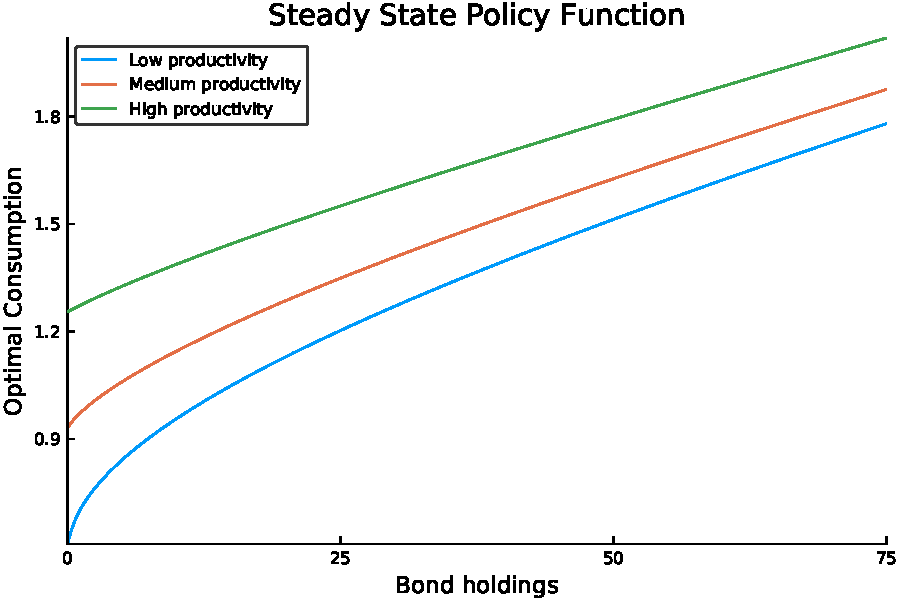
\includegraphics[width=0.7\textwidth]{pol_fn_C.pdf}
\end{figure}

Next, I plot the steady state law of motion for bond holdings; the dashed-line is the 45-degree line. This figure captures the key intuition of why forward guidance is less powerful in MNS's model: highly productive households exhibit precautionary savings behaviour. Precautionary savings tempers the desire to move consumption forward in response to forward guidance.

\begin{figure}[htpb!]
 \centering
        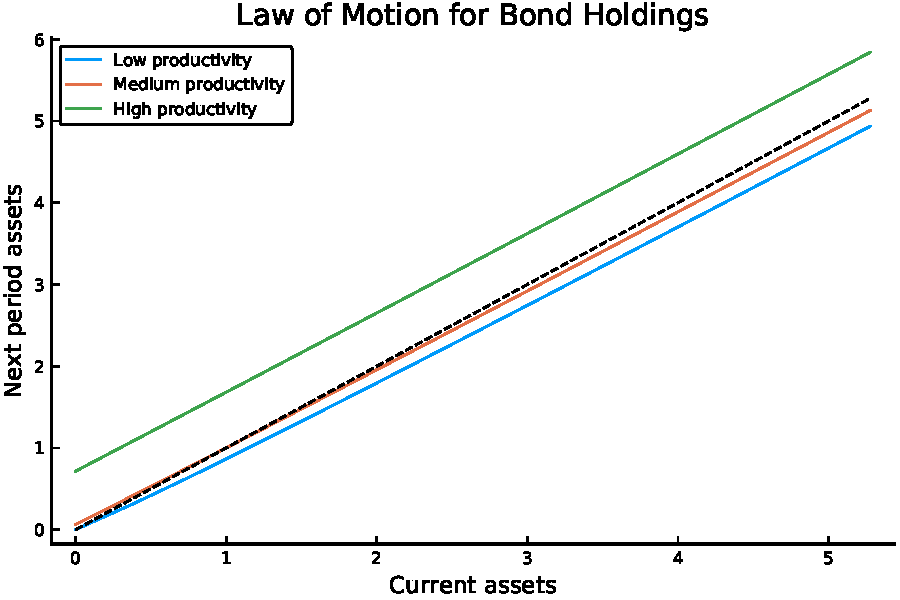
\includegraphics[width=0.7\textwidth]{pol_fn_B.pdf}
\end{figure}

Finally, I plot the steady state distribution of bond holdings (overleaf). Many low- and medium-productivity households are at the borrowing constraint. Furthermore, most high-productivity households have built up a substantial buffer stock of savings.

\begin{figure}[htpb!]
 \centering
        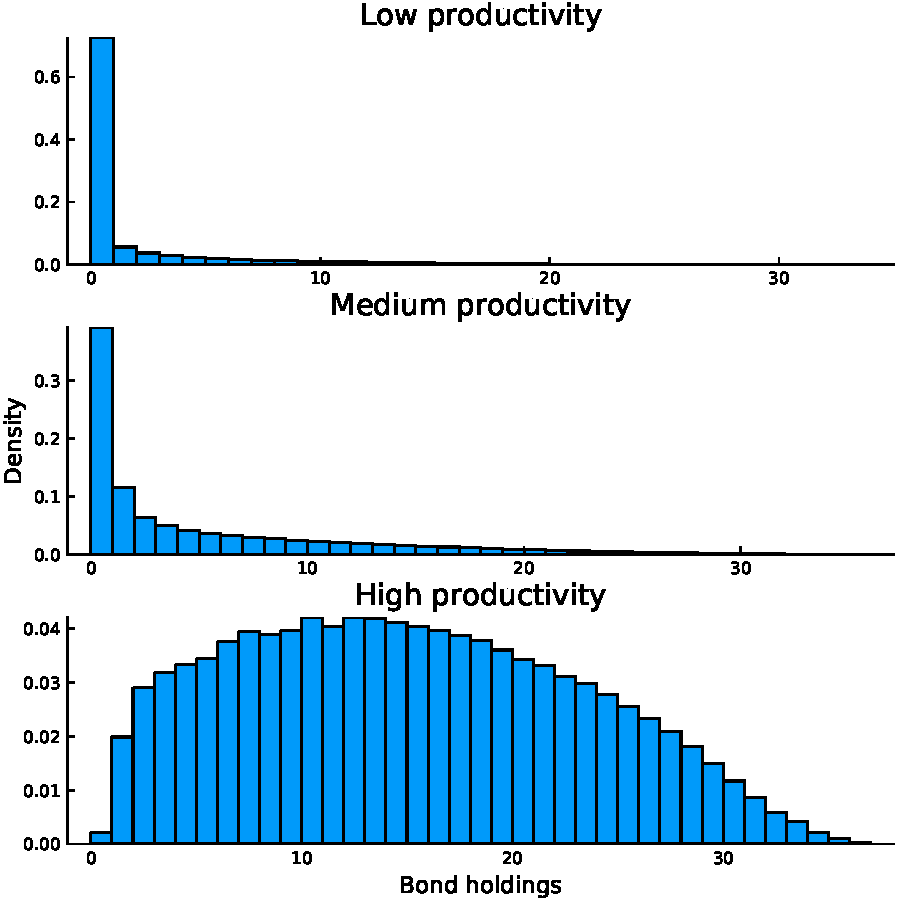
\includegraphics[width=0.7\textwidth]{bonds.pdf}
\end{figure}

\subsection{Problems with my solution}
Although my iterative algorithm converges to something, it turns out that the labor and bond markets don't exactly clear. I get $\bar L = 1.0358$ and $\bar N = \bar C = 1.0368$, which are very close, but not quite equal. Moreover, I get a mean level of bond holdings of 5.95, whereas bond supply is $B = 1.4\times 4 \times \bar C = 5.806$. These small discrepancies may have something to do with the difference between the bond grinds that MNS and I use.\footnote{I use an evenly-spaced bond grid ranging from 0 to 75, with 200 points, while MNS use an unevenly-spaced grid over the same range.}\\

I tried to address this issue by writing another iterative algorithm, which computes the steady state interest rate and wage as well as dividends and taxes. This algorithm gets very close to clearing all markets, but unfortunately never converges. After 100 iterations, I get $\bar r = 0.0053$ and $\bar W = 0.81$, which are slightly above and below their calibrated values in the paper, respectively.

\newpage

\section{Appendix}
\subsection{Endogenous grid method}
EGM is a numerical method for implementing policy function iteration. It starts with the household's Euler equation,
\begin{align}
c_t^{-\gamma} \geq \beta(1+r_t) \sum_{z_{t+1}}\Pr(z_{t+1}|z_t)c_{t+1}^{-\gamma},  \label{eq:hh1}
\end{align}
which holds with equality when the borrowing constraint is not binding. It also uses the intratemporal labor supply condition, which is standard
\begin{align}
\ell_t^\psi &= W_tz_tc_t^{-\gamma}\nonumber \\
\implies  \ell_t&=c_t^{-\gamma/\psi}(W_tz_t)^{1/\psi}\label{eq:hh2}
\end{align}

\subsubsection{Initial guess of the household's policy function}
For the EGM method, I need an initial guess of the policy function. Let's keep this as simple as possible: suppose we start in the steady state and that households consume all of their available resources and save nothing. That is
\begin{align*}
c =  b + \bar Wz\ell - \tau\bar\tau(z) +\bar D
\end{align*}
Substituting the labor supply condition into the above expression, and rearranging a little gives
\begin{align}
c = c^{-\gamma/\psi}(\bar Wz)^{\frac{1+\psi}{\psi}}+ b - \tau\bar\tau(z) +\bar D \label{eq:hh3}
\end{align}
Thus, the initial guess for the policy function, denoted by $g^0(z,b)$, is the level of $c$ that solves (\ref{eq:hh3}). With MNS's calibration, this is just a quadratic equation in $c$ (since $\gamma=\psi=2$), which I can solve easily. So I have an initial consumption level for each $(z,b)$ pair.

\subsubsection{Iterating on the Euler equation}
For starters, assume that the Euler equation holds with equality (I'll deal with the borrowing constraint properly below). Define a grid over values of \textit{tomorrow's} bond holdings $b'$ and call it $B = \{b_1, ...,b_{n_b}\}$, with $b_1 = 0$. The grid of possible productivity draws is $Z=\{z_l, ..., z_{n_z}\}$, and has an associated transition matrix $\mtx{P}$. Then, with my initial guess of the policy function, I can write the Euler as
\begin{align*}
c^{-\gamma} = \beta(1+r) \sum_{z'}\Pr(z'|z)(g^0(z',b'))^{-\gamma}.
\end{align*}
Then, today's consumption is simply
\begin{align}
c = \left( \beta(1+r) \sum_{z'}\Pr(z'|z)(g^0(z',b'))^{-\gamma}\right)^{-1/\gamma} \label{eq:hh4}
\end{align}
Now, recall that the household optimally chooses $b_{t+1}$, while $b_t$ is predetermined. Thus, (\ref{eq:hh4}) gives today's consumption for someone who drew productivity $z$ today, and optimally chose $b'$ for tomorow's bond holdings. So, we can write (\ref{eq:hh4}) as
\begin{align}
\tilde g^0(z,b') = \left( \beta(1+r) \sum_{z'}\Pr(z'|z)(g^0(z',b'))^{-\gamma}\right)^{-1/\gamma} \label{eq:hh5}
\end{align}
I can write (\ref{eq:hh5}) using my grid indicies and the transition matrix
\begin{align}
\tilde g^0(z_i,b_j) = \left( \beta(1+r) \sum_{\ell=1}^{n_z}\mtx{P}_{i\ell} (g^0(z_\ell,b_j))^{-\gamma}\right)^{-1/\gamma} \label{eq:hh6}, 
\end{align}
which gives the optimal policy $c$, for an agent with current productivity $z_i$, and who optimally chooses tomorrow's bond holdings $b_j$. Thus, for each $(z_i,b_j)$ pair I can get the associated optimal consumption today using (\ref{eq:hh6}).\\

Note that I can easily stack (\ref{eq:hh6}) in matrix form. Let $\mtx{G}^0$ be the $n_z \times n_b$ matrix containing our initial guesses of the optimal policy (so $\mtx{G}^0_{ij}$ gives the optimal consumption for state pair $(z_i,b_j)$). Then, the updated guess can simply be computed as
\begin{align*}
\widetilde{\mtx{G}}^0 = \left( \beta(1+r) \mtx{P} (\mtx{G}^0)^{-\gamma}\right)^{-1/\gamma},
\end{align*}
which is essentially what my \verb|Julia| code is doing (note that my \verb|Julia| code actually uses a nested for loop, but I could probably change it to the above matrix code!)\\

Next, I can use the budget constraint to back out \textit{today's} bond holdings $b_t$:
\begin{align*}
b_t = c_t + \frac{b_{t+1}}{1+r_t} -  W_tz_t\ell_t + \tau_t\bar\tau(z_t) - D_t
\end{align*}
Using the intratemporal labor supply condition (\ref{eq:hh2}) to substitute in for $\ell_t$, gives
\begin{align*}
b_t = c_t + \frac{b_{t+1}}{1+r_t} -  c^{-\gamma/\psi}(\bar Wz)^{\frac{1+\psi}{\psi}} + \tau_t\bar\tau(z_t) - D_t
\end{align*}

Using the grid indicies, and my guess for today's consumption, I can write:
\begin{align*}
b^*_{i,j} = \tilde g^0(z_i,b_j) + \frac{b_j}{1+r} - \left(\tilde g^0(z_i,b_j)\right)^{-\gamma/\psi} (\bar Wz_i)^{\frac{1+\psi}{\psi}} + \tau\bar\tau(z_i) - \bar D ,
\end{align*}
where $b^*_{i,j}$ denotes the bond holdings today for a household who gets a productivity draw $z_i$ today, and who optimally chooses tomorrow's level of bond holdings, $b_j$. Then, we can finally define the `endogenous grid' of today's bond holdings (for each level of productivity $z_i$):
\begin{align*}
B_i^* = \{ b^*_{i,1}, ... , b^*_{i,n_b}\}.
\end{align*}
Next, note that for each grid point in $B_i^*$, I have the updated guess of the optimal policy:
\begin{align*}
g^1(z_i,b^*_{i,j}) =  \tilde g^0(z_i,b_j)
\end{align*}
However, the grid points in $B_i^*$ need not (and will not, in general) coincide with the points in the original grid $B$. Thus, to get the updated guesses $g^1(z_i,b_j)$ for each $b_i \in B$ I need to interpolate $g^1(z_i,b^*_{i,j})$, which is pretty straightforward in \verb|Julia|. MNS use a shape-preserving cubic spline, but for now I'll stick with a simple linear interpolation.\\

Now, I need to deal with the borrowing constraint, $b_{t+1} \geq 0$. Recall that $b^*_{i,j}$ is today's bond holdings for someone with current productivity $z_i$ and who optimally chooses $b_j$. Suppose the borrowing constraint binds;  then agent optimally chooses $b_{t+1} = b_j =0$. Thus, from the budget constraint, today's bond holdings are
\begin{align*}
b^*_{i,1} = \tilde g^0(z_i,b_j) - \left(\tilde g^0(z_i,b_j)\right)^{-\gamma/\psi} (\bar Wz_j)^{\frac{1+\psi}{\psi}} + \tau\bar\tau(z_j) - \bar D.
\end{align*}
Recall that $\tilde g_0(z_i,b_1)$ is our guess of optimal consumption today. Accordingly, $b^*_{i,1}$ represents the \textit{highest} level of bond holdings \textit{today} for someone with current productivity $z_i$, such that the borrowing constraint binds. Then, for all grid points $b_j \leq b^*_{i,1}$, when $z=z_i$, the borrowing constraint must bind (i.e. $b_{t+1}=0$). Then, we can use the budget constraint to get the updated guess of today's optimal consumption for constrained agents:
\begin{align*}
g^{1,c}(z_i,b_j) = b_j + \left(g^{1,c}(z_i,b_j)\right)^{-\gamma/\psi} (\bar Wz_i)^{\frac{1+\psi}{\psi}} - \tau\bar\tau(z_i) +\bar D \text{ for all } b_j \leq b^*_{i,1},
\end{align*}
where $c$ superscript denotes `constrained'. Again, with MNS's calibration this is just a quadratic equation.\\

Putting all this together, the updated guess of the optimal policy function is
\begin{align*}
g^1(z_i,b_j) = 
\begin{cases}
\tilde g^0(z_i,b_j) &\text{ if } b_j > b^*_{i,1} \text{ (and appropriately interpolated)}\\
g^{1,c}(z_i,b_j)&\text{ otherwise.}
\end{cases}
\end{align*}






\end{document}
